%!TEX root = ../master.tex
\chapter{Code Overview}\label{ch:codeoverview}
This chapter provides a detailed description of the software code. Figure~\ref{fig:flowchart} provides a simplified overview of the software.

\begin{figure}
\centering
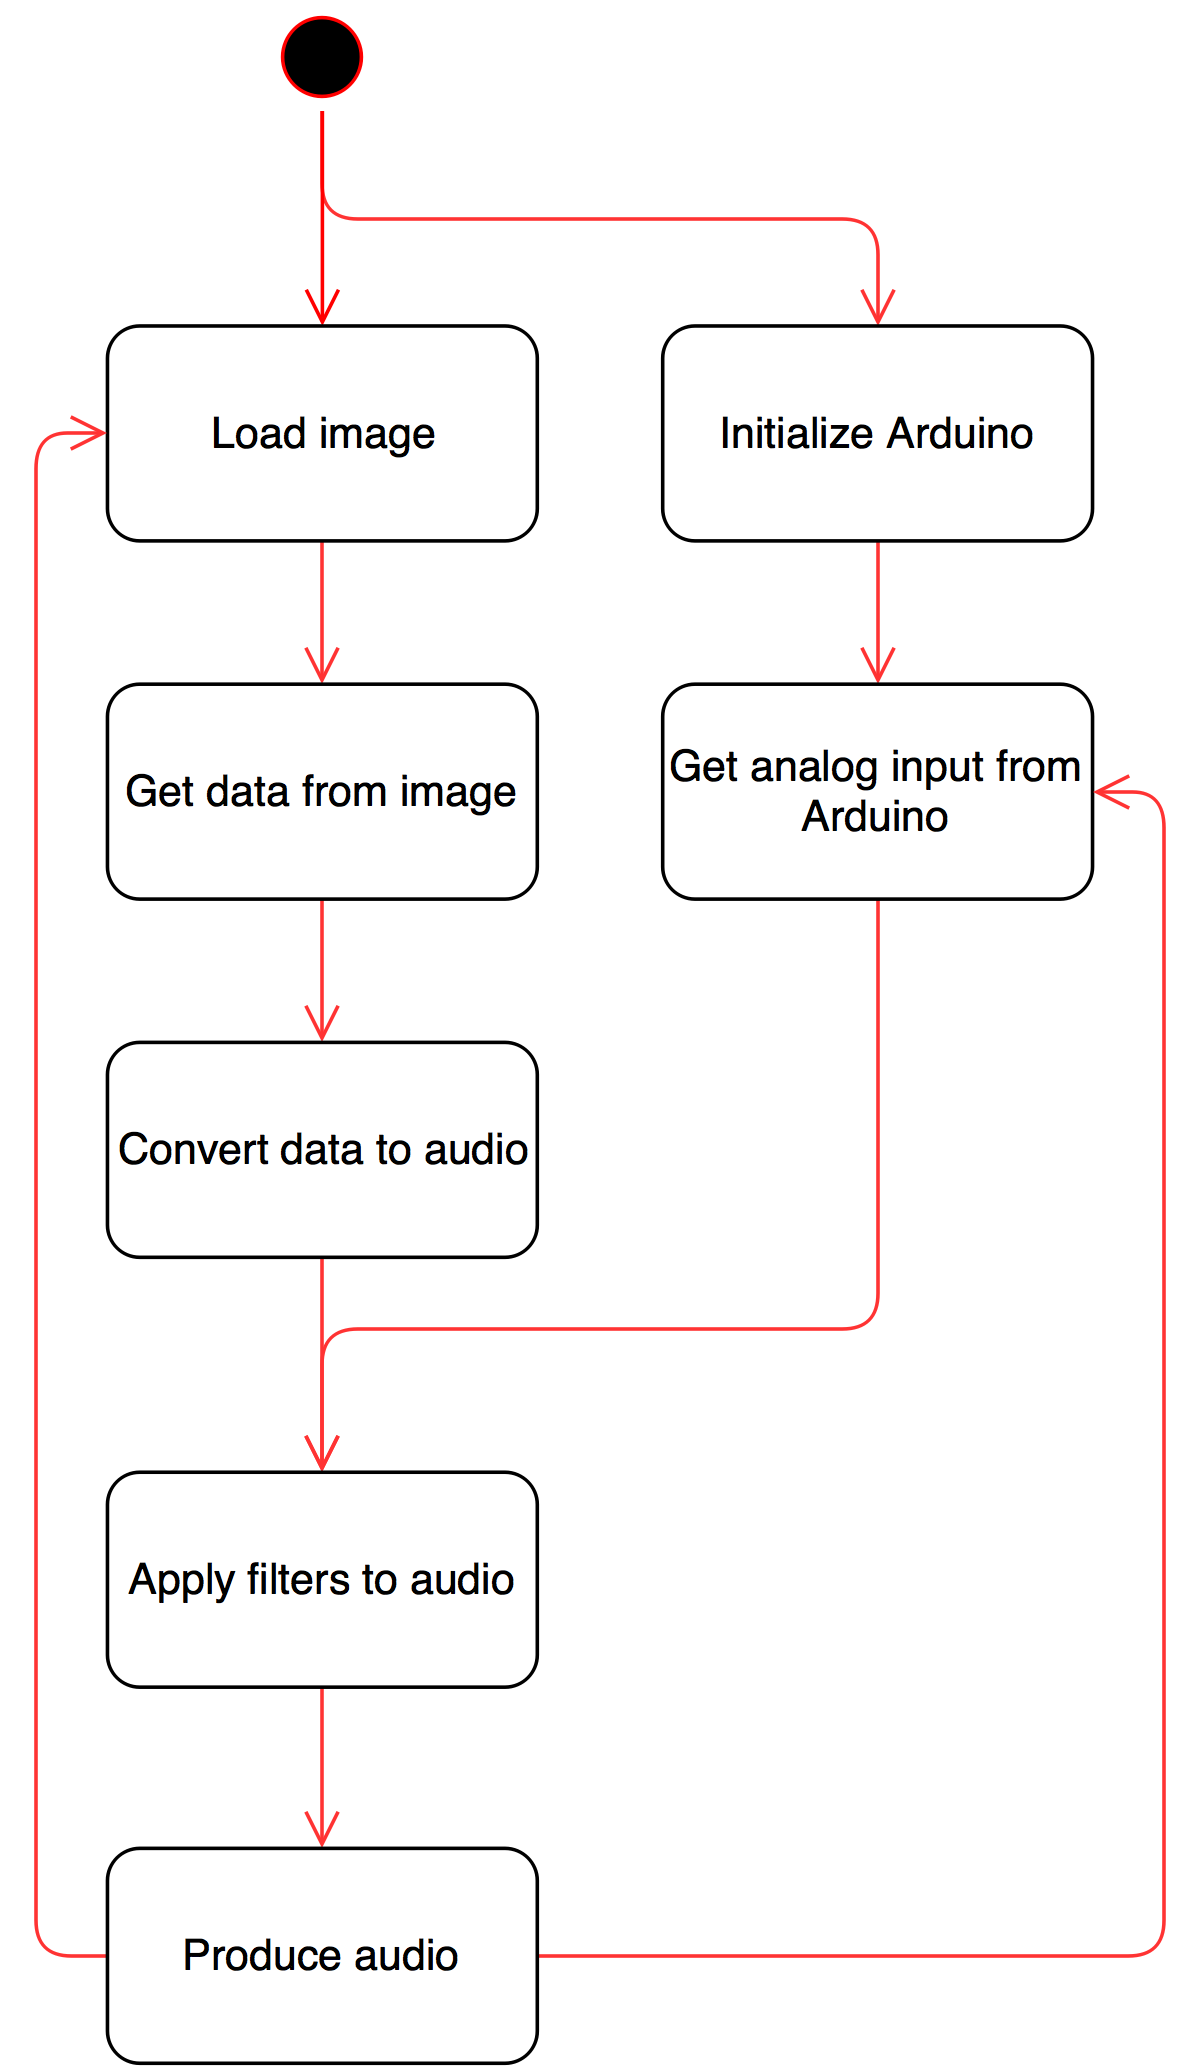
\includegraphics[width=0.5\textwidth]{flowchart}
\caption{Activity diagram showcasing the overall software.}
\label{fig:flowchart}
\end{figure}

\begin{figure}
\centering
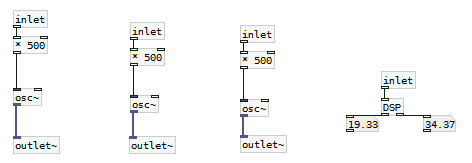
\includegraphics[width=1\textwidth]{Output}
\caption{The contents of \texttt{pd output}.}
\label{Fig:Output}
\end{figure}

\section{Audiolisation code}
When importing pictures into Pure Data a message called \texttt{open} is used. It takes a picture from a specific location and outputs it to \texttt{pix\_image} which is the object that is used for preparing an image for further use. \texttt{pix\_image} sends the image into the \texttt{pix\_draw} which draws the image directly onto the screen. After the images is drawn, it is then sent into the \texttt{pd imageprocessing} patch which can be seen in Figure \ref{Fig:Imageprocessing}. A simplified diagram of this patch can be seen in Figure~\ref{fig:ipflowchart}.

\begin{figure}
\centering
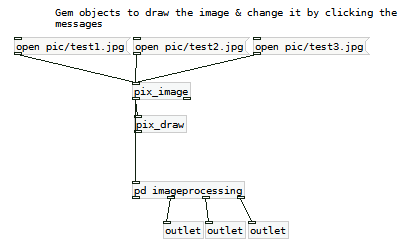
\includegraphics[width=1\textwidth]{Pdpictures}
\caption{The blocks that are responsible for image processing.}
\label{Fig:pdpicture}
\end{figure}

\begin{figure}
\centering
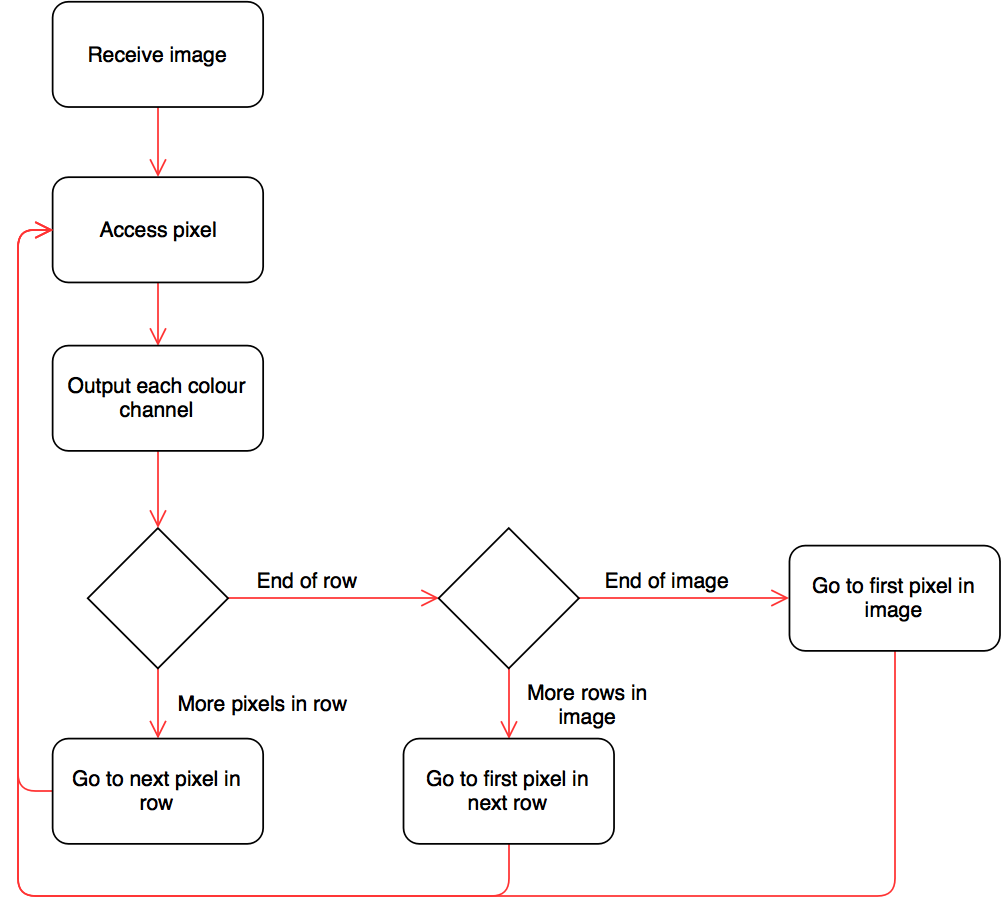
\includegraphics[width=0.5\textwidth]{diagram-ip}
\caption{Activity diagram of the image processing module.}
\label{fig:ipflowchart}
\end{figure}

The inside of the \texttt{pd imageprocessing} patch can be seen on Figure \ref{Fig:Imageprocessing}. A nested for-loop is implemented using an \texttt{expr} function. The for-loop is created using three if-statements, and taking advantage of the dataflow nature of Pure Data, which examines each pixel in the input image according to their x- and y-coordinate.
The loop goes from 0 to 1 with an interval of 0.001. When it reaches 1 it adds 0.01 to the variable \$f2 and resets \$f1 to 0 to start over. When \$f2 hits 1 it resets to 0 and the whole process starts over. The delay is implemented so the program does not preform a stack overflow when handling the if-statements. 
As the if-statements process the data, a set of sliders have been placed to visualise the current pixel position. These sliders move in real time as the image is processed. The information contained in the pixel at current position is outputted to the \texttt{pix\_data} object. It takes a pixel position and the image from \texttt{pix\_image} and outputs the values of the RGB channels into three different numbers boxes which is then outputted out of the \texttt{pd imageprocessing} patch. The output of the \texttt{pd imageprocessing} patch is inputted into the \texttt{pd output} patch. It takes the RGB values and converts it into a cosine wave frequency by multiplying the RGB value by 500 to make sure the frequency is within the range of human hearing \cite{steiglitz1997digital}. It sends the output to the three different filters; bandpass, comb and high-shelf which are explained in Subsection \ref{sub:audiofilters}. The output of the filters bandpass and high-shelf are coefficients, which are used by the biquad to create the filter effect. All three filters are added together and sent to the \texttt{dac~} object which outputs the audio to the speakers. 

\begin{figure}
\centering
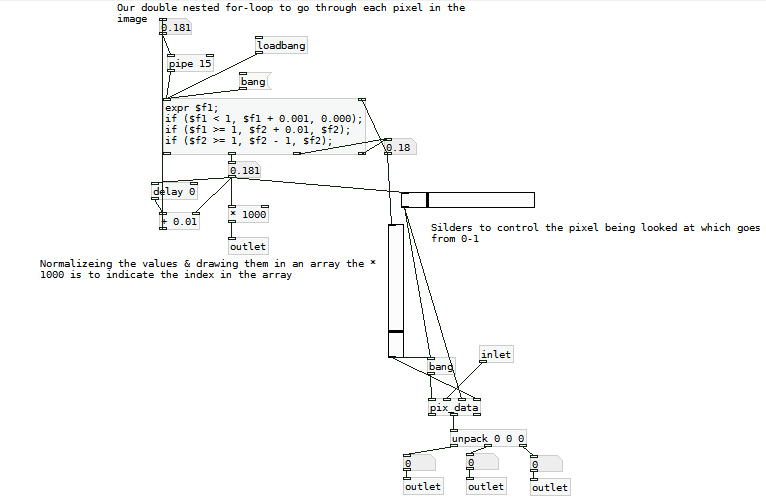
\includegraphics[width=1\textwidth]{Imageprocessing}
\caption{The contents of \texttt{pd imageprocessing}.}
\label{Fig:Imageprocessing}
\end{figure}

\begin{figure}
\centering
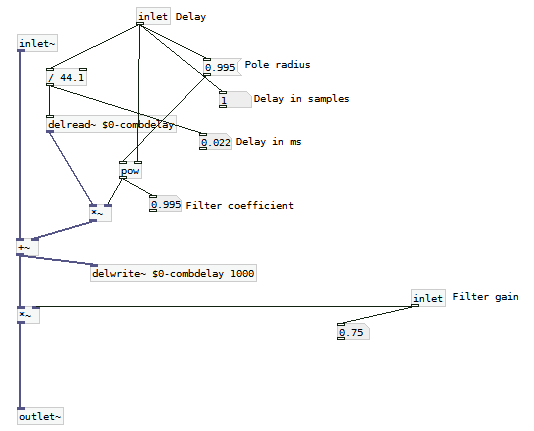
\includegraphics[width=1\textwidth]{Comb_filter}
\caption{The contents of the comb filter patch.}
\label{Fig:Comb_filter}
\end{figure}

\section{Arduino code}
For the Arduino a \texttt{pd arduino} patch has been created, which contains all the objects for the Arduino part of the code. It takes a number and a list of 5 numbers as inputs. The first single number defines which of the computer's serial ports will be used to access the Arduino. The list of numbers defines which analogue inlets are open and which are closed. Each inlet is associated with a position in the list, and the number determines whether a given inlet is active; 1 for active and 0 for inactive. This information is sent to the \texttt{pduino/arduino} object.

\begin{figure}
\centering
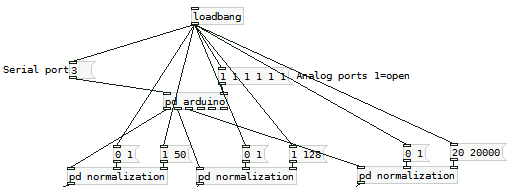
\includegraphics[width=1\textwidth]{Arduino_normalization}
\caption{The Arduino blocks for inputs and outputs.}
\label{Fig:Arudino_normalization}
\end{figure}

The \texttt{pduino/arduino} object sends all of its data into its single outlet. This data contains information from all active in/outlets, digital or analog, as well as information about the Arduino device and how it is performing. The only piece of information the software needs is the data from the analog inlet. The \texttt{route} object is used to filter out all data that does not contain the "analog" label, and then another \texttt{route} object is used to sort the data according to the inlet it originates from. Finally a conversion is made so that the state of each inlet is represented with a floating point number between zero and one. This floating point change when the user operates the slide potentiometer.


\begin{figure}
\centering
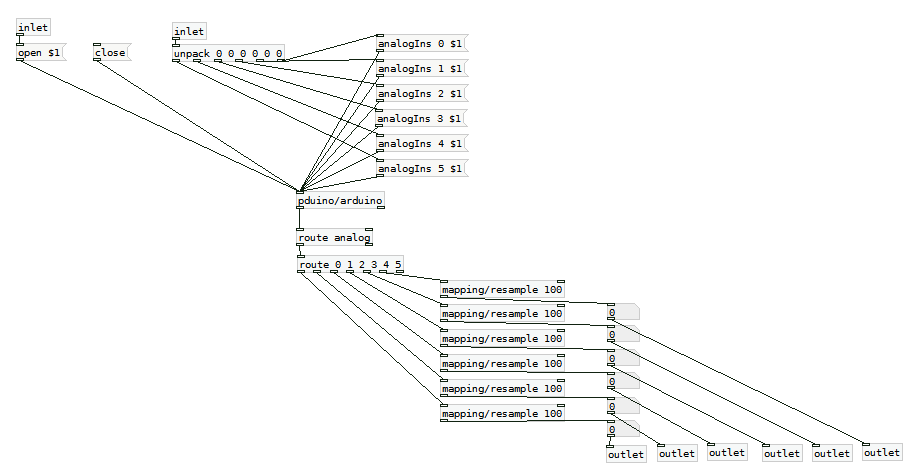
\includegraphics[width=1\textwidth]{Inside_arduino}
\caption{The contents of \texttt{pd arduino}.}
\label{Fig:Inside_arduino}
\end{figure}

The user defined parameters for the filters need coefficients in various ranges. To achieve this, a patch called \texttt{pd normalization} (see Figure \ref{Fig:Normalize}) is used to normalize the numbers from the analog inlets on the Arduino from a range of zero to one to a different range, depending on the filter. \texttt{pd normalization} has three inlets; one for the raw data, one for the original data range, and one for the desired range. The patch then applies the equation $\frac{max'-min'}{max-min}\cdot (data-max)+max'$ where max' and min' make up the desired range, and max and min make up the original range. The result is passed to the outlet which provide one of the filter coefficients for each filter. For the comb filter (see Figure \ref{Fig:Comb_filter}) the coefficient is the delay which altered when the user operates the slide potentiometer. 

\begin{figure}
\centering
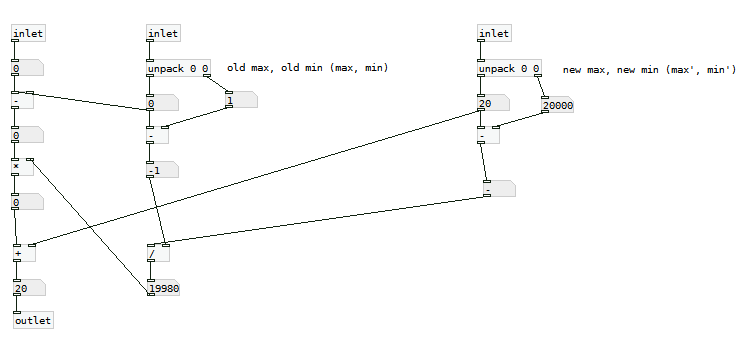
\includegraphics[width=1\textwidth]{Normalize}
\caption{The contents of \texttt{pd normalization}.}
\label{Fig:Normalize}
\end{figure}